\setchapterimage[8.5cm]{desy_blazar}
\setchapterpreamble[u]{\margintoc}
\chapter{Sources of Neutrinos and Gravitational Waves}
\labch{sources}
\begin{fquote}[Winston Churchill][Lady Windermere's Fan][18??]...man will occasionally stumble over the truth, but usually manages to pick himself up, walk over or around it, and carry on. 
\end{fquote}

\begin{fquote}[Arnold J. Rimmer][Red Dwarf][1988] What the hell is a quasar?
\end{fquote}


The origin of the astrophysical neutrino flux discovered by IceCube remains unknown. In this chapter, various potential neutrino sources are discussed, as well as present constraints on the contribution of these sources. Limits have been placed on these source classes by IceCube following the procedure outlined in Chapters \ref{ch:llh} and \ref{ch:neutrino_cosmology}.

Beyond the information presented here, new constraints placed by the author on the population contribution of Tidal Disruption Events (TDEs) and Fast Blue Optical Transients (FBOTs) are outlined in Chapter \ref{ch:results}, and the identification of the TDE AT2019dsg as a likely high-energy neutrino source is outlined in Chapter \ref{ch:bran}.

\section{Galactic neutrino emission}

As introduced in Chapter \ref{ch:theory}, the galactic plane accounts for a significant fraction of EM emission in every photon wavelength, from radio to high-energy gamma rays. It is therefore natural to suspect that the Milky Way might contribute to the astrophysical neutrino flux. Likely sources of galactic neutrinos are primarily those objects detected in gamma rays, such as Supernova Remnants (SNRs), X-ray binaries (XRBs) and Pulsar Wind Nebulae (PWNe) \sidecite{gaisser_95}. In addition, given that the galaxy should act as a target for extragalactic UHECRs and thus produce secondary neutrinos, it is guaranteed that some galactic contribution should be present in the neutrino flux. 

Despite this expectation, to date no significant galactic neutrino excess has been found \sidecite{ic_17_galactic}. Given the position of the galactic centre in the southern hemisphere, where IceCube muon track datasets are less sensitive, IceCube searches are typically conducted using likely-astrophysical cascades. These searches have in some cases been conducted jointly with the northern-hemisphere ANTARES neutrino observatory. At this point, limits on the galactic neutrino flux are beginning to constrain reasonable models of galactic gamma-rays and CRs, including parameters of the popular KRA-$\gamma$ model \sidecite{kra_15}. Given constraints limiting the galactic contribution to less than 14\% of the diffuse flux, we can state with certainty that the astrophysical neutrino flux must be \textbf{predominantly extra-galactic} \cite{ic_17_galactic}. 

Targeted tests were performed on specific galactic objects, but none have identified any significant excess. For example,  study of 23 young supernova remnants, including some with PWNe, limited the catalogue contribution to less than 5.7\% \cite{ic_17_galactic}. A more recent search, targeting only TeV-detected PWNe \sidecite{ic_20_pwn}, constrained their contribution to less than <1.4\% of the total. Various additional studies including composite catalogues of galactic sources have also not revealed significant excesses, see e.g \sidecite{2020PhRvL.124e1103A}.

\section{Active Galactic Nuclei}
\label{sec:agn}

One long-favoured candidate neutrino source class is Active Galactic Nuclei (AGN). These AGN are a subset of the Supermassive Black Holes (SMBHs) believed to be present in the centre of most if not all galaxies. When these SMBHs are  accreting sufficient material to produce significant electromagnetic emission, they are said to be \emph{Active}. As illustrated in Figure \ref{fig:agn_unification}, there are a range of observationally-defined AGN sub-classes \sidecite{2012agn..book.....B}. 

A fraction of AGN launch relativistic jets, which emit strongly at radio frequencies, and thus AGN can be divided into radio-loud or radio-quiet subsets. Radio-quiet AGN are commonly referred to as \emph{Seyfert Galaxies} \sidecite{seyfert_43}. Radio-loud AGN are subclassified as either \emph{blazars}, when observers look directly into the relativistic jet, or \emph{radio galaxies} when the jet is viewed side-on.

There are further categories based on viewing angle. The inner region of an AGN contains fast-moving gas clouds which produce Doppler-broadened emission lines, with this zone dubbed the \emph{Broad-Line Region} (BLR). This BLR is typically surrounded by a dusty torus, which can obscure the BLR when viewed side-on. For AGN where we can see broad lines in optical spectra, we classify them as either Seyfert 1 if radio-quiet, or as broad-line radio galaxies if radio-loud. Conversely, if the BLR is hidden, we have either a radio-quiet Seyfert 2 galaxy or a radio-loud narrow-line radio galaxy (since only narrow emission lines will be visible in the spectra). Seyfert galaxies with intermediate broad-line features can be further quantified as e.g Seyfert 1.8 galaxies \sidecite{osterbrock_81}.

Distinctions of radio galaxies are also made on the basis of morphology, with the Faranoff-Riley classification scheme distinguishing those jets which become dimmer (FR-I) or brighter (FR-II) as the distance from the central AGN increases \sidecite{fanaroff_riley_74}. In general, these morphological effects are proxies for jet luminosity, with FR-II being more luminous than FR-I, hence the brighter jet extremities. Analogously, blazars can be sorted by their Spectral Energy Distribution (SED) properties into either \emph{Flat-Spectrum Radio Quasars} (high-luminosity) or \emph{BL-Lacs} (low-luminosity), with the latter class named after nearby blazar \emph{BL-Lacertae} \sidecite{95_agn_unification}.

Though AGN unification now appears natural, the historical process of discovery based on observations has left several anomalous or arbitrary classifications. Early observations of AGN identified them as compact objects of unknown origin which bore some similarity to stars. They were thus dubbed \emph{quasi-stellar objects}, or QSOs, with \emph{quasi-stellar radio objects} dubbed \emph{quasars}. 

One misfit in the standard AGN unification scheme is the phenomenon of \emph{Changing-look AGN} (CLAGN), namely those AGN which appear to rapidly transition from one class to another \sidecite{shappee_clagn}. The mechanism that causes the changing look remains unconfirmed, but explanations include variation in line-of-sight obscuration or transient accretion events such as a tidal disruption event (see section \ref{sec:tde}).

\begin{figure}[!ht]
	\centering \includegraphics{sources/agn_unification}
	\caption{Unified model of AGN, with classification depending on observer viewing angle, taken from \cite{2012agn..book.....B}.}
	\label{fig:agn_unification}
\end{figure}

\subsection{Neutrinos from Blazars}
Blazars, with their highly-beamed emission from relativistic jets, were one of the first proposed sources of high-energy neutrinos, predating the discovery of the astrophysical neutrino flux by two decades \sidecite{mannheim_93}. Blazars have revealed a characteristic SED with two characteristic "humps", as shown in Figure \ref{fig:blazar_sequence}. While there is consensus that the lower-energy hump likely arises from synchrotron emission,  the higher-energy one has been explained both by leptonic and hadronic models. Neutrino emission would be expected for hadronic models, though the extent would also depend on the availability of a suitable target for the accelerated hadrons to collide with.???

\begin{figure}[!ht]
	\centering 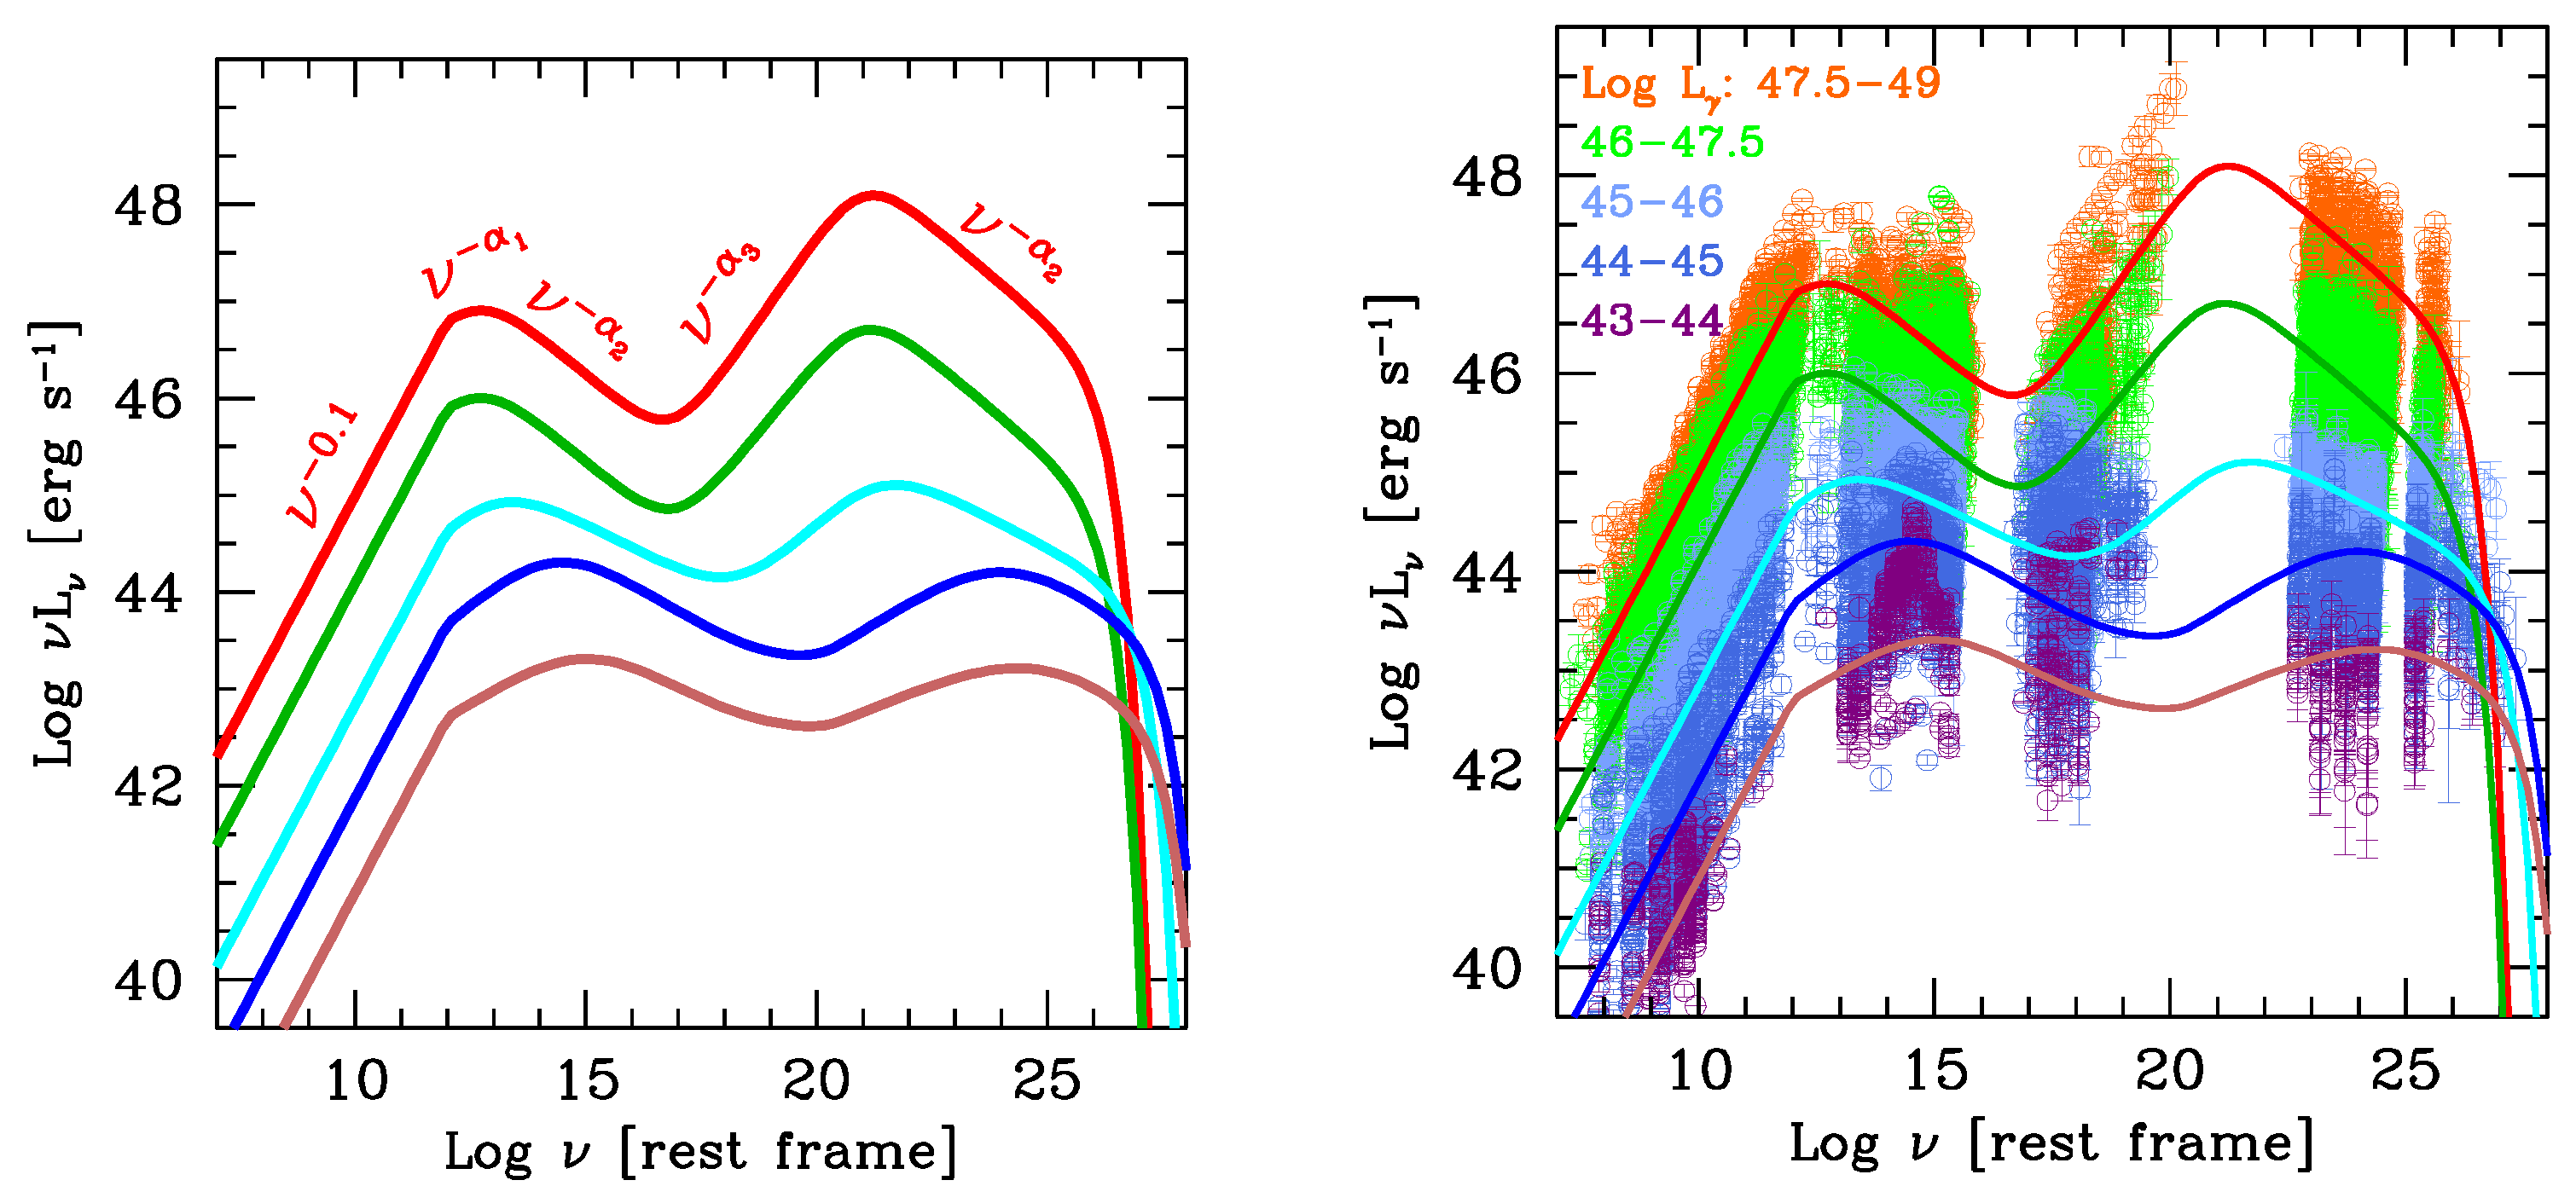
\includegraphics{sources/blazar_sequence}
	\caption{Characteristic blazar SEDs as a function of luminosity, from \cite{16_blazar_sequence}.}
	\label{fig:blazar_sequence}
\end{figure}

The second SED peak typically falls in the MeV-TeV range, and blazars are thus routinely detected by $\gamma$-ray telescopes. Since launch in 2008, the comprehensive $\gamma$-ray sky survey by the Fermi Large Area Telescope (Fermi-LAT) has now detected 3137 blazars \sidecite{fermi_4fgl}. Indeed, it is now known that blazar emission dominates the high-energy gamma-ray sky. Modelling of the "Extragalactic Gamma-Ray Background" (EGB) reveals that $\sim$ 50\% of all gamma-ray emission in the Fermi range is produced by blazars, of which $\sim$ 70\% belongs to Fermi-detected blazars \sidecite{15_fermi_egb}.  

Imaging Air Cherenkov Telescopes (IACTs) have also confirmed that blazars are extremely bright at TeV gamma-rays, beginning with Markarian 421 as the first extragalactic TeV source \sidecite{92_mrk421_tev}. However, at TeV energies and above, $\gamma$-rays are increasingly likely to interact with photons from the diffuse Extragalactic Background Light (EBL), leading to an attenuation of emission from distant objects \sidecite{10_ebl}. Though only nearby blazars can thus be detected at TeV energies, it is generally assumed by extrapolation that more distant blazars are also likely TeV-emitters.

 Given the simultaneous production of gamma-rays with neutrinos in hadronic interactions, it is natural to suspect that bright gamma-ray sources, namely blazars, may additionally be neutrino sources. This hypothesis has been tested repeatedly by IceCube, and under the assumption of a linear proportionality ("$\gamma$-ray weighting"), the contribution of all blazars has been constrained to less than 10\% of the astrophysical neutrino flux \sidecite{ic_blazar_17}. Though only 862 blazars from the older Fermi 2LAC catalogue were tested, the limit is corrected to additionally account for the contribution of unresolved blazars. 
 
 A second analysis with the same catalogue of 2LAC blazars, using an agnostic equal-weight-per-blazar assumption ("equal weighting"), found that the catalogue contributes less than 20-30\% of the total, without placing any constraint on the contribution of non-catalogue blazars \cite{ic_blazar_17}. 
 
 More generally, the $\gamma$-ray weighting result and generic spectral considerations have \textbf{strongly constrained scenarios in which the neutrino production can be reliably traced by $\gamma$-ray emission} \sidecite{murase_hidden_sources_16}. That does not mean that blazars cannot produce a substantial neutrino flux, but $\gamma$-bright blazars must not dominate it. Recent theoretical work on blazar neutrino emission have instead focussed on evading both this and the equal-weighting constraint through models which predict a substantial contribution from unresolved and lower-luminosity blazars \sidecite{palladino_19}.
 
 \subsection{TXS 0506+056}
 
 However, this conclusion was challenged by observations of high-energy neutrino IC170922A, found in spatial and temporal coincidence with a bright gamma-ray flare from blazar TXS 0506+056 \sidecite{2018Sci...361.1378I}, (see also Chapter \ref{ch:realtime}). A likelihood analysis correlating high-energy neutrinos with the monthly gamma-ray lightcurves of Fermi blazars led to the disfavouring of a chance coincidence at the level of $3 \sigma$. This result implied that, rather than the average gamma-ray flux, high-energy neutrinos might instead be correlated with instantaneous $\gamma$-ray blazar flux. 
 
 Prompted by this observation, the IceCube collaboration conducted a time-dependent search for archival neutrino emission from the direction of TXS 0506+056 \sidecite{IceCube:2018cha}, and identified an additional signal-like cluster of 13 neutrinos in 2014-15 with a significance of $3.5 \sigma$. However, in contrast to the detection of IC170922A, this "neutrino flare" was not accompanied by any significant contemporaneous gamma-ray activity \sidecite{garrappa_19}. TXS 0506+056 thus presented a somewhat contradictory picture, with both pieces of evidence challenging to interpret in a unified framework. 
 
Because the association of IC170922A and TXS 0506+056 was promptly identified \sidecite{fermi_txs_atel_17}, there were extensive contemporaneous multi-wavelength observations of the flare \cite{2018Sci...361.1378I}. Theoretical attempts to model the arrival of IC170922A generally arrived at the same conclusion, namely that without violating observational constraints the probability of detecting a neutrino alert is generally smaller than $\sim$ 15\% \sidecite{gao_txs_19}. However, this is nonetheless consistent with a physical association after accounting for the substantial Eddington Bias expected for a single neutrino detection \sidecite{2019A&A...622L...9S} (see also Chapter N).
 
On the other hand, attempts to model the neutrino flare were significantly more challenging because the implied neutrino flux during the flare period was extremely large. Moreover, the Eddington bias should be minimal for a detection with 13 neutrinos. Despite relatively weak observational constraints for the 2014-15 period there have been no successful models capable of producing 13 neutrinos without violating the multi-wavelength observations \sidecite{rodrigues_19}.

Assuming that all three pieces of evidence (the stacking limit, IC170922A and the neutrino flare) are indeed correct, it is difficult to reconcile them. One vital question is whether TXS 0506+056 belongs to some "neutrino blazar" sub-population. Given that the probability of detecting a high-energy neutrino may already be $\sim$1-15\% from TXS 0506+056 alone, the IC170922A association can easily be reconciled once accounting for Eddington Bias from even a moderately-sized "neutrino blazar" population of $\sim$10-100 objects. The coincidence with a gamma-ray flare may indicate that neutrino luminosity is correlated to gamma-ray luminosity after all, but in order to reconcile a sufficient flux for neutrino alert with the the existing stacking limit, the neutrino blazar population must not include those nearby/bright $\gamma$-ray blazars which dominated the stacking limit \cite{ic_blazar_17}. Satisfying that condition, IC170922A and the stacking limit can clearly be understood coherently.

However, complications arise when trying to also accommodate the neutrino flare, over and above the immediate inability for theorists to model it. Were such emission replicated for a population covering just 5\% of all blazars, the diffuse astrophysical neutrino flux would be saturated \sidecite{halzen_19_txs}. But, in order to do so with violating the equal-weight stacking limit, neutrino emission would also need to be heavily biased towards $\gamma$-dim blazars. More generally, given that the flare was not accompanied by significant gamma-ray emission, it supports the idea that neutrino emission is not correlated to instantaneous gamma-ray flux. Such an interpretation is inconsistent with the original evidence to support TXS 0506+056 as a neutrino source, namely that a high-energy neutrino was detected coincident with a gamma-ray flare.

Alternatively, it may be possible that one piece of evidence is somewhat incorrect or misinterpreted. The stacking limit itself may be overly conservative, because it is sensitive to the impact of unmodelled systematic uncertainties in event reconstruction (see Chapter N). Another possibility is that the timing of IC170922A may in fact have been coincidental, while the neutrino flare may also have represented random temporal clustering. Given the degree to which searches for time-varying and steady neutrino sources are correlated, it is possible that TXS 0506+056 is instead a steady neutrino source, which by random chance exhibited some weak structure in the temporal distribution of neutrinos. One further possibility is that the neutrino flare could perhaps be a random data fluctuation, an interpretation which is supported by the lack of robustness of the excess to variations of data selection and reconstructions methods CITE.

Given the puzzling nature of TXS 0506+056, further evidence of neutrino emission will undoubtedly be required to firmly resolve the cumulative blazar neutrino flux. In any case, \textbf{it is challenging to conceive of scenarios in which the entire astrophysical neutrino flux is produced by blazars}, leaving the door open to contributions from other source classes.

\subsection{Neutrinos from AGN}

Models of neutrino emission from accretion-disk shock-acceleration in AGN emerged even before those models of AGN jets \sidecite{stecker_91}. These models are generally much harder to test, because AGN are vastly more numerous than blazars, leading to a much more diffuse astrophysical neutrino flux. 

Nonetheless, IceCube has recently tested neutrino correlations using samples of more than 30000 radio galaxies, and identified a significant excess. This excess was found to be robust across two catalogue compilation methods, with both results consistent in implying that \textbf{AGN cores contribute substantially to the diffuse astrophysical neutrino flux}. While most significant result is just 2.96 $\sigma$ post-trial (3.16 $\sigma$ pre-trial), the second catalogue has an additional pre-trial significance of 2.01 $\sigma$. Though both catalogues are intended to test the same hypothesis, the source overlap is just 13\%, so that the second catalogue provides \emph{significant independent evidence supporting the association}. However, given the degree of uncertainty in the associated neutrino flux, there is plenty of scope for further neutrino flux contributions from additional neutrino sources.

\section{Core-Collapse Supernovae}
\label{sec:ccsn}

\begin{marginfigure}
	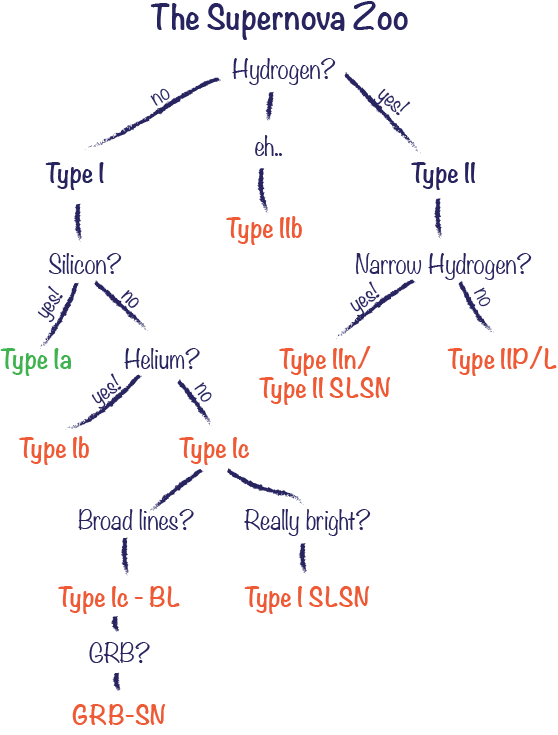
\includegraphics{sn_zoo-1}
	\caption{An overview of the current supernova classification scheme, from N.}
	\label{fig:snzoo}
\end{marginfigure}

Supernovae, the explosive death of stars, are perhaps the best-studied phenomenon in astronomy. They are traditionally classified based on observed properties, rather than intrinsic physical attributes. An overview of a classification scheme is given in Figure \ref{fig:snzoo}. The most fundamental distinction is in explosion mechanism, with Type Ia SNe occurring due to thermonuclear explosions while all other classes are believed to arise from stellar core collapse. 

Further classifications are made based on the presence of various emission line, which can reveal properties of the progenitor star or local environment. Additional classifications can be made on the basis of photometric properties, such as SN IIP which exhibit lightcurve plateaus, or IIL which have linear lightcurve decays. 

An additional category of supernovae has been recently observed, identifiable by their atypical brightness. So-called Superluminous supernovae (SLSNe) were initially classified as any SNe with an absolure magnitude brighter than -21 mag. However, in recent years, increased study has led to a spectroscopic classification being favoured, with some dimmer objects in the range $-20 < M < -21$ also being accepted. 

\subsection{Neutrinos from CSM-interaction}

One proposed mechanism for neutrino production is through the collision of SN ejecta with dense cicumstellar material (CSM), dubbed the \emph{CSM-interaction} mechanism \sidecite{murase_csm_sn_11}. For those SNe which occur in these dense environments, the CSM interaction typically produces characteristic spectra with narrow lines, leading to the distinct subclass of SN Type IIn. 

The timescales for neutrino production are uncertain, but could last for dozens to hundreds of days as the interaction continues. An IceCube search for neutrino emission from these Type IIn supernovae on these timescales did not reveal any significant correlation \sidecite{Stasik2018Search}, and their contribution was limited to 27.5\%  of the diffuse neutrino flux under the assumption that all IIn are neutrino standard candles. 

Supernovae of other types may also have some degree of CSM interaction, for example IIP \sidecite{iip_csm_14}. This hypothesis was also tested by IceCube, under the assumption that all IIP are neutrino standard candles, and the class was found to contribute less than n\% of the total \cite{Stasik2018Search}. This weaker constraint primarily arises from the much higher rate of IIP supernovae than IIn (see Chapter \ref{ch:nu_cosmology}). There have been no comparable studies to date on SLSNe with evidence of interaction, so their contribution remains unconstrained.

\subsection{Supernova Jets and Long Gamma-Ray Bursts}

It is now understood that some supernovae launch relativistic jets, and that these can generate extremely luminous $\gamma$-ray transients known as Long Gamma-Ray Bursts (LGRBs), which have long been proposed as a source of neutrinos \sidecite{waxman_bahcall_97_grb}. Though these LGRBs were initially discovered independently, subsequent observations have since established that they arise from Type Ic supernova which also exhibit broad spectral lines (Ic-BL supernovae) \sidecite{98_grb_sn}. The jet itself is launched at the time of supernova explosion, leading to a GRB if aligned towards the Earth. Subsequently, a Type Ic supernova appears, with the high-velocity jet ejecta creating the characteristic broad spectral lines. However, while GRB-less Ic-BL supernovae would generally be expected due to jet misalignment, radio observations indicate that many Ic-Bl supernovae do not launch relativistic jets at all CITE.

In any case, neutrinos would only be expected for those jets which align towards Earth. The most reliable confirmation of an aligned jet is the corresponding detection of a LGRB, with neutrino emission typically predicted to occur during the so-called "prompt phase" of $\gamma$-ray emission ( $\sim$100s). 

IceCube has undertaken numerous searches for neutrino emission, but has so far observed no correlation. Owing to the similar physical conditions, these neutrino searches have typically not distinguished LGRBs from the "Short Gamma-Ray Bursts" (SGRBs) which arise from neutron star mergers (see Section \ref{sec:ns_mergers}). Prompt emission from GRBs is particularly favourable for neutrino detection, because the brief and well-defined search period greatly reduces the expected background for such searches. This scenario is indeed one of the most-constrained by IceCube, which current limits restrict to less than 0.4\% of the astrophysical neutrino flux \sidecite{ic_grb_17}. 

\begin{figure}[!ht]
	\centering 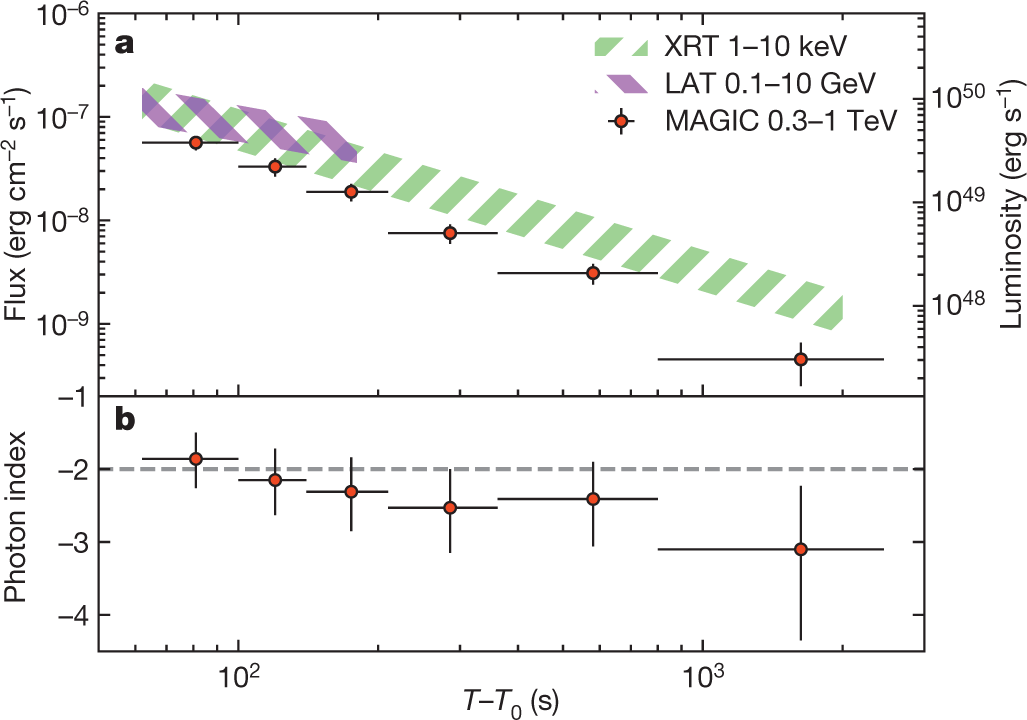
\includegraphics{sources/magic_grb}
	\caption{Detection of a GRB afterglow at TeV energies, from \cite{magic_grb_19}.}
	\label{fig:magic_grb}
\end{figure}

Our understanding of LGRBs has recently expanded further \sidecite{mirzoyan_grb_19}, with the discovery of VHE gamma-ray emission from a GRB reported by the MAGIC collaboration. This was followed by the announcement of a second VHE GRB detection by the HESS collaboration \sidecite{hess_grb_19}. Both were long GRBs, with the VHE detection coinciding with the well-known "GRB afterglow" typically detected in X-ray/optical wavelengths (see Figure \ref{fig:magic_grb}). While the HESS GRB was particularly bright, the MAGIC detection was coincident with an unexceptional afterglow, suggesting that VHE emission may be common in long GRBs \sidecite{magic_grb_19}.

The timescales for this emission, extending as much as N days after prompt phase indicates that high-energy processes extend throughout the so-called "afterglow phase". consequently there is renewed focus on potential neutrino afterglow  emission, which is significantly less-constrained. One previous Icecube analysis limited the GRB afterglow  contribution to <38\% of the total \sidecite{grb_afterglow_thesis}.

\subsection{Choked Jets and Low-Luminosity Gamma-Ray Bursts}

The same Type Ic-BL supernovae have also been associated with low-luminosity GRBs (llGRBs)  \sidecite{07_llgrb}, a distinct subclass of GRBs that are more numerous but intrinsically far dimmer than their high-luminosity counterparts. It is now thought that llGRBs arise when a jet does not successfully escape the star, but is instead smothered by the intervening material before reaching the star's surface \sidecite{nakar_15_llgrb}. Instead, a mildy relativistic shock propagates through surrounding material before ultimately reaching the surface, emitting wide-angle high-energy emission in a process known as \emph{shock breakout}. This scenario is illustrated in Figure \ref{fig:grb_diagram}.

\begin{figure}[!ht]
	\centering \includegraphics{sources/grb_diagram}
	\caption{Illustration of long GRBs and low-luminosity GRBs, from \cite{nakar_15_llgrb}.}
	\label{fig:grb_diagram}
\end{figure}

Though the gamma-rays are trapped, any neutrinos would still be capable of escaping the star, giving an alternative \emph{choked-jet neutrino production} mechanism \sidecite{senno_choked_jets_16}. In comparison to LGRBs, the choked jets may ultimately be brighter neutrino sources, because protons accelerated by the jet would be trapped within the envelope and efficiently produce neutrinos via pp interactions \cite{nakar_15_llgrb}. Much like for LGRBs, these neutrinos would still be expected shortly after supernova explosion, and again only if the choked jet was aligned towards Earth. However, with enhanced neutrino production and an intrinsically higher occurrence rate, llGRBs might contribute substantially more to the diffuse neutrino flux than LGRBs. 

Unfortunately, due to their low luminosity, LLGRBs are detected with much lower efficiency than LGRBs, leaving only a handful of known examples. Given this, targeted stacking searches of llGRBs are significantly less powerful. However, for this case, generic searches for short-scale neutrino multiplets provide constraints on the contribution of such a population. From constraints on minute-scale astrophysical neutrino clustering, LLGRBs are known to contribute less than ???\% \sidecite{Strotjohann2020Search}.

As an alternative method, neutrinos could be correlated directly with SN Ic-BL, because these supernovae are detected with much higher efficiency than llGRBs. This scenario is however particularly difficult to test, because the alignment of a choked jet cannot be measured, so it is impossible for us to say which supernovae should or should not produce neutrinos. Furthermore, unless shock breakout is serendipitously observed, the time of supernova explosion can only be estimated to within a few days, rather than the $\sim$100s window for a GRB detection. To date, there has been no dedicated IceCube search for neutrinos correlated directly with Ic-BL supernovae. Though one study found no significant evidence of correlation with supernovae of Types Ib and Ic, that sample was dominated by non-Ic-BL supernovae \cite{Stasik2018Search}. 

Check

\section{Neutron Star Mergers}
\label{sec:ns_mergers}

An alternative source of neutrinos may be neutron star mergers, a source class which has recently been detected by the LIGO-Virgo Collaboration (LVC) gravitational wave detectors \sidecite{lvc_gw170817}. Neutron star mergers are divided by the composition of the binary pair that merges, either Binary Neutron Stars (BNS mergers) or the merger of a neutrino star and a black hole (NSBH mergers). Both classes have now been detected with GW detectors.

\subsection{Short Gamma-Ray Bursts}

Short Gamma-Ray Bursts (SGRBs) are now known to arise from relativistic jets launched during the merger of binary neutron stars \sidecite{lvc_gw170817}, following the coincident detection of BNS GW170817 and GRB170817A. This coincident detection, illustrated in Figure \ref{fig:gw170817}, confirmed long-standing theories about the neutron star origin of SGRBs \sidecite{grb_bns_92}. Whether NSBH mergers also produce GRBs remains an open question.

\begin{figure}[!ht]
	\centering 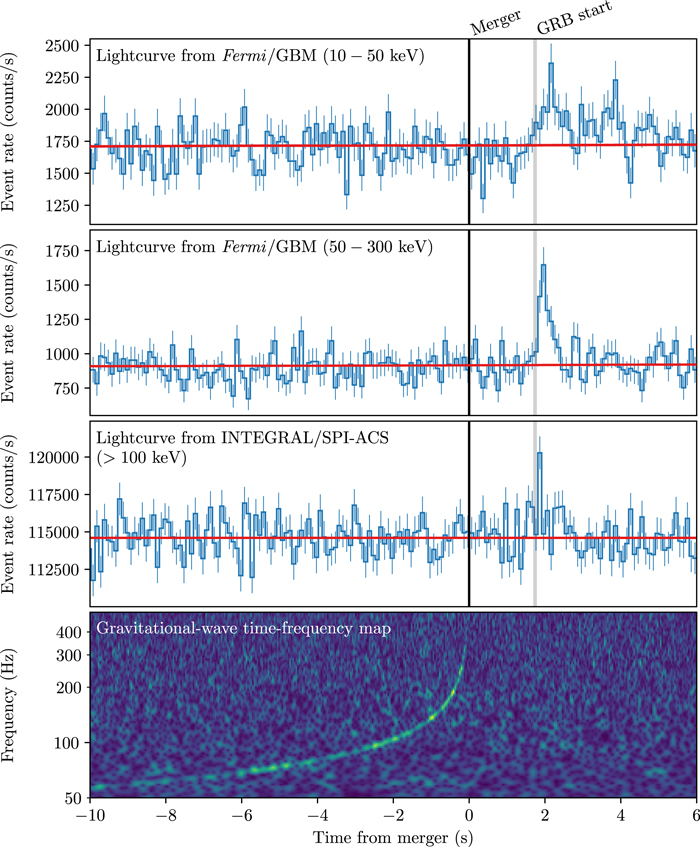
\includegraphics{intro/apjlaa920cf2_lr.jpg}
	\caption{The detection of a binary neutron star merger with photons (upper 3 panels) and gravitational waves (lower panel) , from \cite{grb170817}.}
	\label{fig:gw170817}
\end{figure}

Observations of GRB170817A revealed that it was particularly underluminous relative to most short GRBs, a fact later explained by comprehensive observations and modelling which confirmed an off-axis jet geometry \sidecite{gw170817_jet_18}. Given the relatively narrow jet opening angle, it is expected that the majority of future binary neutron star mergers detected by LIGO will not have detectable GRB counterparts.

Much like the LGRBs described in Section \ref{sec:ccsn}, SGRBs were initially identified as promising neutrino source candidates \cite{waxman_bahcall_97_grb}. However, no significant evidence for correlation has yet been found. The combined constraint on SGRBs+LGRBs, limiting their contribution to less than 0.4\% of the total diffuse neutrino flux, is the most stringent placed on neutrinos from NS mergers \cite{ic_grb_17}. An independent search for neutrino emission coincident with LIGO-detected BNS mergers also found no significant excess, though no limit was placed on the overall contribution of BNS or NSBH mergers to the diffuse neutrino flux \sidecite{icrc_hussain_19}.

\subsection{Kilonovae}

\section{Binary Black Hole Mergers}

The first direct evidence for the existence of Gravitational Waves (GWs) was first provided by the detection of a Binary Black Hole (BBH) merger during LIGO's first observing run (O1) \sidecite{ligo_bbh_16}. With subsequent enhancements to detector sensitivity,  LIGO has to date detected a total of 10 high-significance BBH mergers across the first two observing runs, in collaboration with the Virgo detector for O2 \sidecite{gwtc_1}. 

In general, BBH mergers themselves are not expected to produce either electromagnetic counterparts or neutrino emission. However, depending on the BBH environment, electromagnetic radiation and particle acceleration could occur under certain conditions \sidecite{murase_bbh_16}. One suggested scenario is that black hole binaries may preferentially form in the accretion disks of AGN, in which case shocks could generate detectable counterparts. Indeed, a candidate EM counterpart has now been reported for one of the BBH candidates reported by LIGO during O3, further supporting this theory \sidecite{graham_gw_20}.

However, a test for neutrino emission from GW triggers from the first two LIGO observing runs revealed no significant neutrino emission from BBHs \sidecite{ic_gw_20}. Given that neutrino emission would only be expected for a subset of BBH mergers, it is difficult to extrapolate from a non-detection to a limit on the overall contribution of BBH mergers to the astrophysical neutrino flux. Only the identification of electromagnetic counterpart can establish that a BBH merger belongs to this neutrino-capable subset, and no search for neutrino emission has yet been published for the sole candidate member of this class \cite{graham_gw_20}.

\section{Fast Radio Bursts}

A relatively recent astrophysical phenomenon are Fast Radio Bursts (FRBs), a class of bright millisecond radio bursts \sidecite{lorimer_07}. The vast majority of FRBs appear to have an extragalactic origin. While most FRBs appear to be transient events, there are now multiple examples of repeated FRBs from the same location \sidecite{frb_repeater_16}. Though a variety of models exist to explain the origin of FRBs, no consensus has yet emerged. Repeating FRB 121102 was however localised to a low-metallicity dwarf galaxy, which are also known to preferentially host SLSNe and LGBRs (see Section \ref{sec:ccsn}), suggesting that these classes of transient may be connected \sidecite{petroff_frb_19}. 

Regardless of their origin it is clear that the detection efficiency of FRBs remains extremely low, with an estimated all-sky rate of one detectable FRB per minute, of which only a handful per year are actually detected \cite{petroff_frb_19}. As a class of energetic transients, models gave suggested that FRBs may be sources of UHECRs, and thus neutrinos \sidecite{frb_nu_model}. However, because the fraction of population neutrino emission that is expected to come from detected FRBs is so low (see Chapter \ref{ch:neutrino_cosmology}), the neutrino flux contribution of the FRB population remains unconstrained \sidecite{ic_frb_20}.

The detection of the first galactic FRB (FRB 200428) coincident with magnetar SGR 1935+2154 confirmed that at least some FRBs are indeed produced by magnetars \sidecite{bochenek_20}. While the fluence of FRB 200428 was extremely large due to its proximate origin, the intrinsic energy released was orders of magnitude lower than extragalactic FRBs. No neutrino emission was detected by IceCube \sidecite{atel_frb_sgr}, strongly con straining any standard-candle FRB contribution to the diffuse neutrino flux. However, for scenarios in which neutrino luminosity is not uniform across FRBs, a significant contribution cannot be excluded.

\section{Starburst Galaxies}
Another possibility is that the astrophysical neutrino flux is produced by a large population of steady sources, and is thus truly a \textbf{diffuse} astrophysical neutrino flux. One case would be for neutrino production in Starburst Galaxies, which has been suggested in various models \sidecite{loeb_sbg_16}. Such a scenario is unfavourable for identification against an isotropic neutrino background, and in this case it is unlikely that IceCube would have sufficient sensitivity to identify the neutrino flux origin. However, given that pionic neutrino production should be accompanied by gamma-rays, constraints can instead be derived from analysis of the non-blazar component of the gamma-ray flux \sidecite{bechtol_sbg_17}.

\section{Tidal Disruption Events}
\label{sec:tde}

Tidal Disruption Events (TDEs) occur when a star passes close to a super-massive black hole (SMBH) \sidecite{rees_tde_88}. The strength of tidal force exerted by the SMBH on the star can exceed the self gravity holding the star together, in which case the star disintegrates, and is then said to have been \emph{tidally disrupted}. Part of the stellar debris falls back to the black hole and is ultimately accreted, a process which generates an electromagnetic signature known as a Tidal Disruption Flare (TDF).

Early modelling \sidecite{evans_89} suggested that mass fall-back rate in a TDE should follow a characteristic t$^{-5/3}$ power law, which might lead in some circumstances to TDFs with corresponding t$^{-5/3}$ lightcurves. This observational signature led to the identification \sidecite{komossa_99} of the first candidate TDEs, detected in X-ray with significant transient emission.

Even before the routine detection of TDEs in sky surveys, the potential contribution of TDEs to the UHECR flux was identified \sidecite{farrar_09}. Following the discovery of \emph{Swift J1644+57}, it is now known that some TDEs also launch relativistic jets \sidecite{bloom_11}, in a transient analogue to the blazar jets introduced in Section \ref{sec:agn}. This further expanded the possible avenues for particle acceleration in TDEs.

TDEs are now commonly detected in surveys such as ZTF (see section N) \sidecite{van_velzen_20}, enabling population science to be done on a homogeneous sample . Some tentative spectral classes have now been identified, analogous to those of CCSNe (see Section \ref{sec:ccsn}), which correlate to host galaxy and photometric properties of TDEs. 

Theory

As part of this thesis, the first search for neutrino emission from TDEs was undertaken (see Chapter \ref{ch:results}). The contribution of Jetted TDEs was limited to n\%, while that of non-jetted TDEs was limited to N\%.  This thesis also outlines the first observational evidence supporting TDEs as hadronic sources, with the identification of AT2019dsg as a likely neutrino source (see Chapter \ref{ch:Bran}).

\section{Fast Blue Optical Transients}

A new population of objects known as Fast Blue Optical Transients (FBOTs) has recently been identified \sidecite{drout_fbot}. While most FBOTs were detected at high redshift, particular interest in FBOTs has increased following the detection of a particularly nearby and bright example AT2018cow \sidecite{Margutti:2018rri}. This promptly-identified transient at a distance of just 60 Mpc provided a rich multi-wavelength dataset, upon which most FBOT understanding is now based. The exact mechanism behind FBOTs remains open to debate, with varying interpretations such as TDEs with an Intermediate-Mass Black Hole, extreme supernovae or a Magnetars \sidecite{Perley:2018oky}. In any case, they are a class of bright transients which exhibit substantial non-thermal emission, making them interesting candidates for neutrino emission.

Some degree of neutrino emission has been predicted for FBOTs, but an IceCube detection would only be expected for AT2018cow-like objects located at distances less than $\sim$15 Mpc \sidecite{fang_fbot_19}. In this thesis, the first dedicated search for neutrino emission from AT2018cow on month-long timescales was performed (see Chapter \ref{ch:results}). No significant excess was identified, and the cumulative contribution of FBOTs to the diffuse neutrino flux was limited to less than N\% of the total.

\section{Summary}

All of this limits outlined above are listed in Table \ref{tab:source_limits}.

\begin{table*}[]
	\centering
	\begin{tabular}{|c c c c c c|} 
		\hline
		Source Class & Limit Type & Fraction & $\phi_{0}$ at 100 TeV & Weighting & Reference\\ 
		&&[\%]&[GeV$^{-1}$ cm$^{-2}$ s$^{-1}$]&&\\
		\hline
		Galactic Plane & - & 14.0 &  3.8 $\times 10^{-18}$  & Fermi-LAT $\pi_{0}$ model &\cite{ic_17_galactic}\\
		SNR (TeV-detected) & Catalogue & 5.7 & 1.6  $\times 10^{-18}$ & Equal & \cite{ic_17_galactic}\\
		PWN (TeV-detected) & Catalogue & 1.4 & 4.5 $\times 10^{-19}$ & Equal &  \cite{ic_20_pwn}\\
		\hline
		Blazar (Fermi-detected) & Catalogue & 27&7.6 $\times 10^{-18}$& Equal & \cite{ic_blazar_17}\\
		Blazar (all) & Population &10&2.8 $\times 10^{-18}$& L$_{\nu} \propto$ L$_{\gamma}$& \cite{ic_blazar_17}\\
		AGN Cores & Population &?&& L$_{\nu} \propto$ L$_{x}$&\\
		SN IIn & Population & 27.5 &7.7 $\times 10^{-18}$&Standard Candle&\cite{Stasik2018Search}\\
		SGRB+LGRB (Prompt) & ? & 0.4 &1.1 $\times 10^{-19}$?&Equal?&\cite{ic_grb_17}\\
		FRB & Population & 100.0 & 2.8 $\times 10^{-17}$& Equal & \cite{ic_frb_20}\\
		TDE (Jetted) &Population&& &Standard Candle & This work\\
		TDE (Non-jetted) & Population &26.& &Standard Candle & This work\\
		FBOT & Population &&& Standard Candle & This work\\
		\hline
	\end{tabular}
	\caption{Summary of the limits on each source class, including results from Chapter \ref{ch:results}. Those limits marked \emph{Population} represent limits on the total contribution of a source class, while \emph{catalogue} limits constrain only those sources tested. Fractions are given as a percentage of the diffuse flux measured in X, with sky-integrated normalisation of 2.81 $\times 10^{-17}$ GeV$^{-1}$ cm$^{-2}$ s$^{-1}$ at 100 TeV, and spectral index $\gamma=2.5$}
	\label{tab:source_limits}
\end{table*}{}

\begin{figure}[!ht]
	\centering 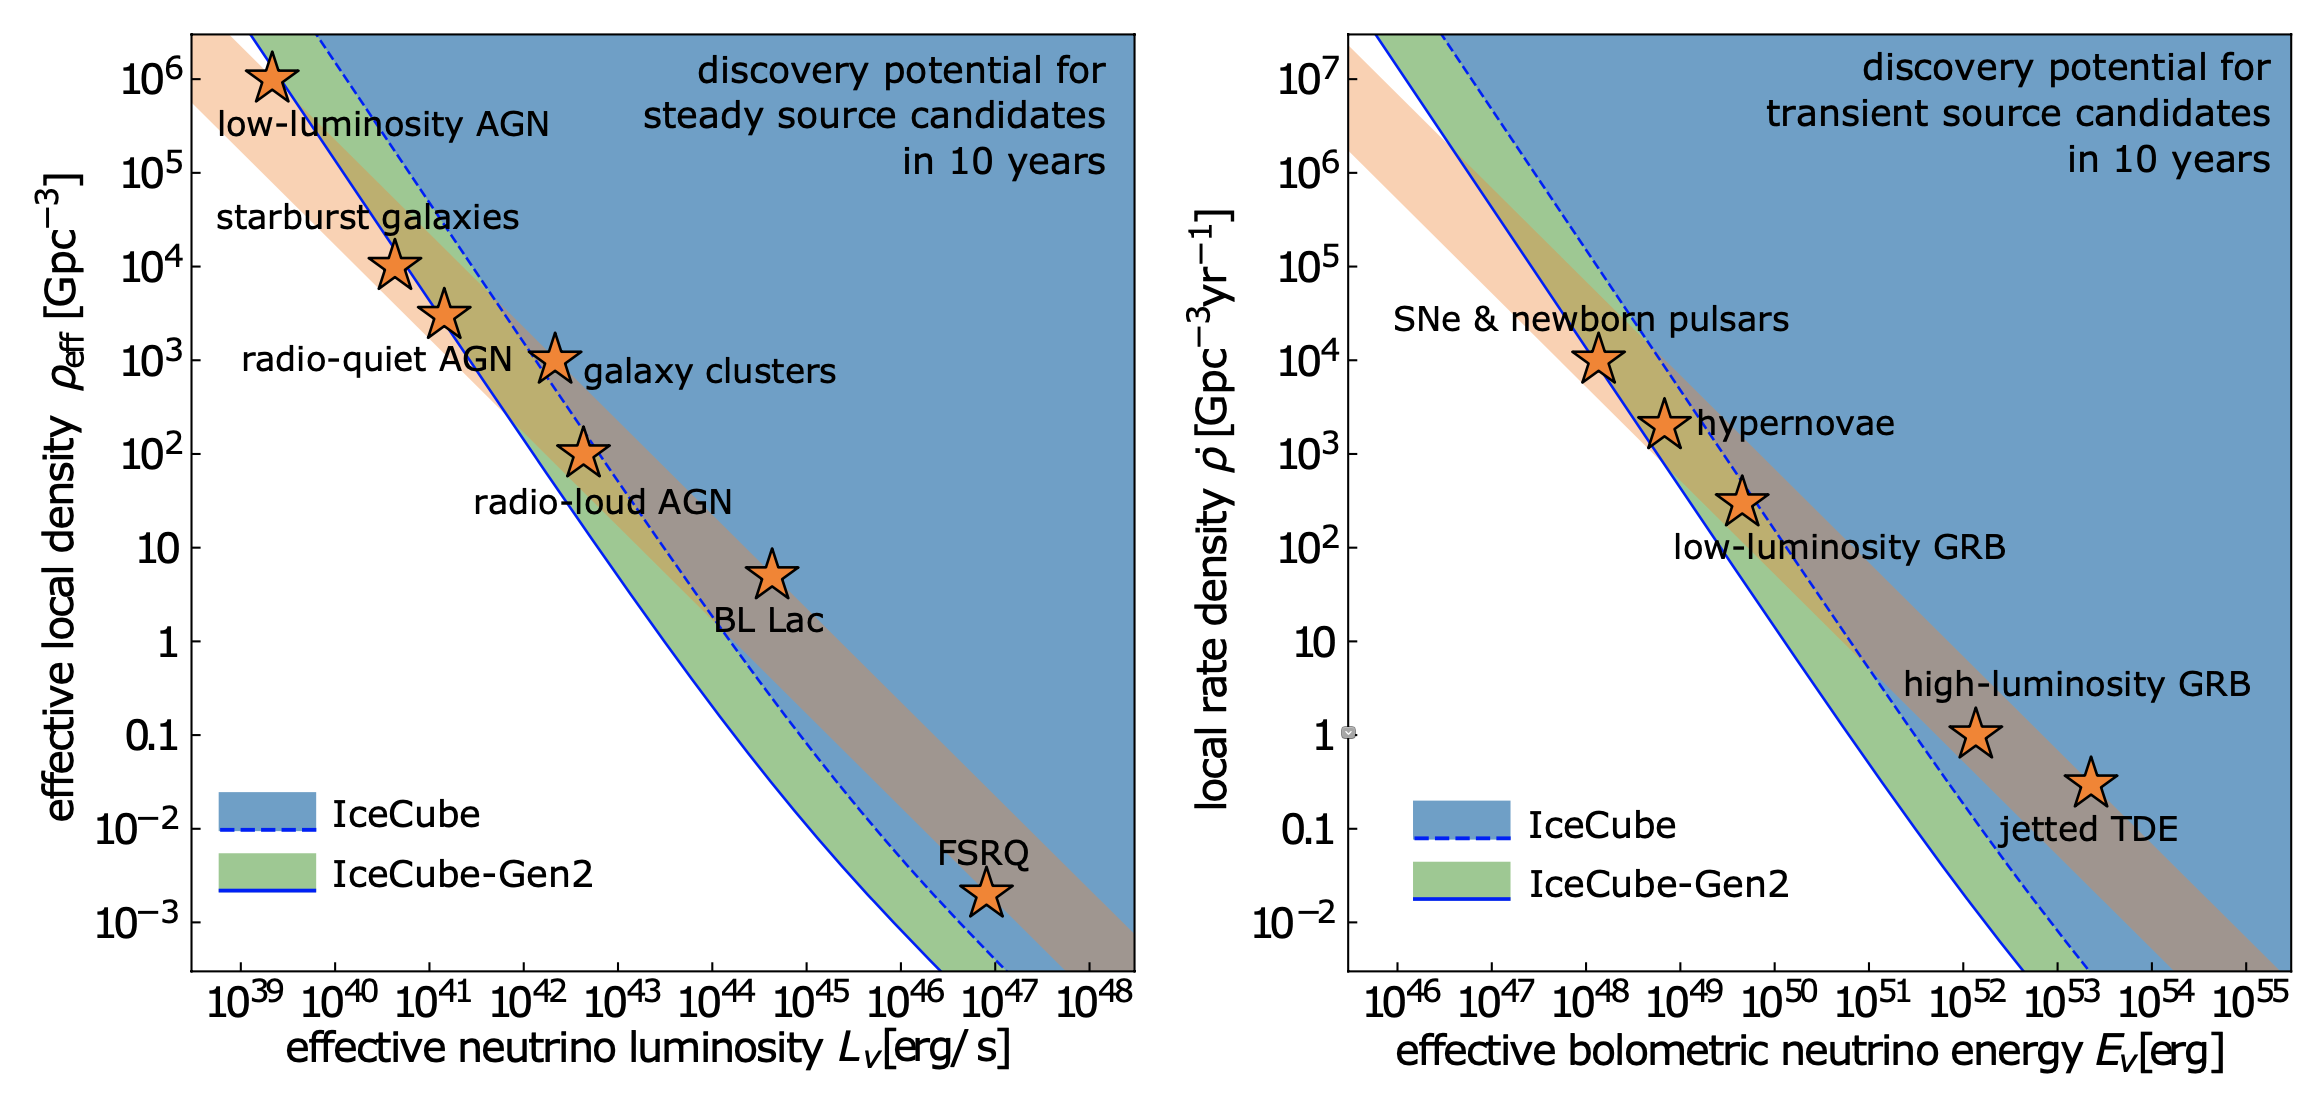
\includegraphics{sources/kowalski_plot}
	\caption{\emph{Kowalski Plot} illustrating source densities and luminosities, from \cite{ic_gen2_20}.}
	\label{fig:kowalski_plot}
\end{figure}

Kowalski plot